\documentclass[a4paper,12pt]{book}
\usepackage[utf8]{inputenc}
\usepackage{amsmath,amssymb,latexsym}
\usepackage{graphicx,subfigure}
\usepackage{tcolorbox}
\usepackage{wrapfig}
\usepackage{rotating}
\usepackage[margin=2.5cm]{geometry}
\newtheorem{Equation}{\indent Equation}[section]
\textwidth=6in
\renewcommand{\baselinestretch}{1.5}

\begin{document}

\author{Zachary Matheson}
\title{Everything you wish you'd known when you STARTED your PhD}
\date{Revised February 2017}

\frontmatter
\maketitle
\tableofcontents

\mainmatter
\chapter{Pairing in Nuclear Theory}

\maketitle
There are several different ways to include pairing correlations in nuclear structure calculations, many of which are based on the BCS theory of superconductors. In it, nucleon pairs can be described as quasiparticles in a nuclear superfluid. Here I will describe three different approaches for describing nuclear structure which account for pairing, each with varying degrees of generality.

\section*{BCS Theory and HF+BCS (\cite{suhonen2007nucleons,Anguiano2013})}
One way to include pairing correlations is to solve the Hartree-Fock equations and add BCS on top. This method is called HF+BCS and it does a fair job of describing nuclei near the valley of stability, but gets progressively worse the further from stability you get (see \cite{Anguiano2013}).

Basically the idea is that you use HF to take you from a system with a whole bunch of interdependent particles, which each obey a one-body Hamiltonian piece AND a two-body Hamiltonian piece, to an alternate basis in which you basically only have a one-body Hamiltonian. Then, in that basis, you solve the BCS equations on top, so you're doing BCS on a basis that doesn't exactly describe the real interaction Hamiltonian but is close enough to the real thing.

Another way of saying it is that the HF equations give you single-particle wavefunctions, in the basis which most closely approximates/diagonalizes the [two-body] Hamiltonian. So it's sort of a fictitious basis, in that your Hamiltonian is not \textit{really} diagonal, but it's as good as you're gonna get. That's what the variation does - you're varying the ground state energy according to the coefficients which give you the most ideal linear combination of starting basis functions (harmonic oscillator or whatever). But the main idea is this: that you pretend your two-body Hamiltonian is actually a one-body Hamiltonian, diagonalize it, and make the error in your approximation as small as possible.

For the next step, when you add in the BCS, you typically make (at least for even-even nuclei) the ground state ansatz $|BCS\rangle = \prod_{k>0}(u_k+v_k a_k^\dagger a_{\bar{k}}^\dagger)|0\rangle$, which doesn't conserve particle number (in fact, it's a linear superposition of pairs starting from zero pairs all the way up to $\frac{A}{2}$ pairs), but I guess it's close enough. Then you typically enforce particle number conservation some other way, perhaps by adding a Lagrange multiplier.

Next you take your pairing Hamiltonian, which I suppose would include your mean-field, now one-body Hamiltonian (which stands in for the two-body Hamiltonian you had before you performed Hartree-Fock), and you add in a new two-body potential, which this time represents the effect of pairing. Then you perform a Hartree-Fock-style calculation all over again, essentially just doing another Hartree-Fock calculation on top of your original one, except that this time you might probably have an extra Lagrange multiplier constraint in your Hamiltonian. It doesn't change anything substantial but it's good to keep in mind. There are probably other ways of constraining particle number, too, like Lipkin-Nogami, but I'm not too sure how those work.

Some other things to keep in mind:
\begin{itemize}
\item You can still think of your system in terms of the HF-basis real particle wavefunctions $a_k^\dagger |0\rangle$, with $|BCS\rangle = \prod_{k>0}(u_k+v_k a_k^\dagger a_{\bar{k}}^\dagger)|0\rangle$. Or, to simplify the math, you can invent a new "quasiparticle" such that $|BCS\rangle = \prod_{k}\alpha_k^\dagger|0\rangle$. This trick is called the Bogoliubov transformation and it looks like this:

\begin{eqnarray}
\alpha_k^\dagger = u_ka_k^\dagger-v_ka_{\bar{k}} \label{quasiparticle1}\\
\alpha_{\bar{k}}^\dagger = u_ka_{\bar{k}}^\dagger+v_ka_k \label{quasiparticle2}
\end{eqnarray}
\item A pairing gap $\Delta = 0$ seems to mean there is no energy associated with pairing. All pairs are formed below the Fermi surface, because why on Earth wouldn't they? It's free! Whereas a nonzero pairing gap means there is some energy associated with forming a pair. So the probability of forming pairs is less than one below the Fermi surface, but there's also a possibility that pairs might form outside the Fermi surface. The pairing gap basically defines how far outside the Fermi surface you can go (see p 233 of \cite{ring1980nuclear}, for ex., or p 13 of \cite{Balbuena2003}).
\item You could also do the BCS calculation using single-particle states derived from a phenomenological potential. You'd sacrifice some accuracy but gain some speed \cite{Anguiano2013}.
\end{itemize}

\section*{Hartree-Fock-Bogoliubov (HFB)  (\cite{ring1980nuclear,Balbuena2003})}
In HF theory, you find the eigenfunctions of the one-body Hamiltonian which most closely resembles the actual two-body Hamiltonian. The basic idea to HFB is that in HFB you do basically the same thing, except you can't ignore two-body interactions because of pairing. So I guess in a way you sort of find the eigenfunctions of the two-body Hamiltonian which most closely resembles the actual four-body Hamiltonian. There's a little bit more subtlety than that, because the pairing correlations mean the particles are related somehow, but that's not a bad way to envision it, because one quasiparticle has a $U$ term, which corresponds to adding a particle, and a $V$ term, which does the opposite - so it's like creating a pair all at once (see equation \ref{HFBqp})! In reality, each HFB quasiparticle is a sum of such terms, but you get the idea. In some sense, one quasiparticle $\sim$ two real particles.

By way of comparison to HF+BCS, which is a two-step process, HFB just does both steps at once to give you a single set of quasiparticle wavefunctions, instead of one set of single-particle wavefunctions based on another set of wavefunctions. The approximation in the end is better, but it is more computationally intensive than HF+BCS.

Let's see how this calculation is to be done. Suppose our Hamiltonian is:

\begin{equation}
\hat{H}=\sum\limits_{i,j} t_{ij} \hat{c}_i^\dagger \hat{c}_j + \frac{1}{4}\sum\limits_{i,j,m,n} \bar{v}_{ijmn} \hat{c}_i^\dagger \hat{c}_j^\dagger \hat{c}_n \hat{c}_m
\end{equation}

As mentioned before, let us make the following Bogoliubov transformation to make the math simpler:

\begin{equation}
\left(\begin{array}{c}
\hat{\beta} \\
\hat{\beta^\dagger}
\end{array}\right)
= \left(\begin{array}{cc}
U^\dagger & V^\dagger \\
V^\dagger & U^\dagger
\end{array}\right) \left(\begin{array}{c}
\hat{c} \\
\hat{c^\dagger}
\end{array}\right) \label{HFBqp}
\end{equation}

\noindent Now the Hamiltonian looks like this:

\begin{eqnarray}
\hat{H} = \hat{H}_0 + \sum\limits_{i,j}\hat{H}_i,j\beta_i^\dagger\beta_j + \sum\limits_{i<j}(\hat{H}_{i,j}\beta_i^\dagger\beta_j^\dagger + h.c.) + \hat{H}_{int} \nonumber\\
= \hat{H}_0 + \hat{H}_{11} + \hat{H}_{20} + \hat{H}_{40} + \hat{H}_{31} + \hat{H}_{22}
\end{eqnarray}

\noindent where $h.c.$ is the hermitian conjugate of the previous term and the term $\hat{H}_{nm}$ contains all terms with $n$ quasiparticle creation operators and $m$ annihilation operators. We'll lump the terms with 4 creation/annhilation operators into a single term $\hat{H}_{int}$, which we'll assume is small and thus ignore (sort of like the term $V(r)-\sum_{i,j}V(r_i,r_j)$ from regular Hartree-Fock theory). Let us constrain the average particle number by adding in a Lagrange multiplier term $\lambda N$. Then we vary the total energy with respect to $U$ and $V$ (which are matrices):

\begin{equation}
\delta E' = \langle\Phi_0|\hat{H}-\lambda\hat{N}|\Phi_0\rangle
\end{equation}

After that, it's really just algebra. The variation leaves some ambiguity still in the choice of $U$ and $V$, so we will choose them to make $\hat{H}_{20}=0$ and $\hat{H}_{11}$ diagonal. Additionally, the solution will look nicer if we introduce the following two densities, the traditional single-particle density from Hartree-Fock $\rho$ and a pairing tensor called $\kappa$:

\begin{eqnarray}
\rho_{ij} = \langle\Phi_0|\hat{c}_j^\dagger\hat{c}_i|\Phi_0\rangle = (VV^T)_{ij} \\
\kappa_{ij} = \langle\Phi_0|\hat{c}_j\hat{c}_i|\Phi_0\rangle = (VU^T)_{ij}
\end{eqnarray}

We can make things look \textit{even nicer} if we introduce the following notation representing the mean field $\Gamma$ and the pairing field $\Delta$:

\begin{eqnarray}
\Gamma_{kl} = \sum_{i,j} \bar{v}_{kjli}\rho_{ij} \\
\Delta_{kl} = \frac{1}{2}\sum_{i,j} \bar{v}_{klij}\kappa_{ij}
\end{eqnarray}

After we make all these substitutions, the Hamiltonian looks like:

\begin{equation}
\hat{H}-\lambda\hat{N} = \sum\limits_{i,j}\left(\left(t_{ij} + \frac{1}{2}\Gamma_{ij} - \lambda \right) \rho_{ji} + \frac{1}{2}\Delta_{ij}\kappa_{ji}^* \right) + \sum_{i}E_i \hat{\beta}_i^\dagger\hat{\beta}_i + \hat{H}_{int}
\end{equation}

\noindent where $\hat{H}_{int}$ contains all the terms with four creation/annhilation operators and $\sum_{i}E_i \hat{\beta}_i^\dagger\hat{\beta}_i$ is the diagonal form of $\hat{H}_{11}$.

Finally, putting everything back in terms of the real particle creation and annhiliation operators $c_i^\dagger$ and $c_i$ (and then dropping those in favor of their coefficients), we get the Hartree-Fock-Bogoliubov equations in their most familiar form (setting $h=\epsilon+\Gamma$):

\begin{equation}
\left(\begin{array}{cc}
h-\lambda & \Delta \\
-\Delta^* & -(h-\lambda)^*
\end{array}\right) \left(\begin{array}{c}
\hat{U_k} \\
\hat{V_k}
\end{array}\right)
= E_k\left(\begin{array}{c}
\hat{U_k} \\
\hat{V_k}
\end{array}\right)
\end{equation}

The case of rotating nuclei is interesting because experimental moments of inertia of deformed nuclei are found to be 2-3 times larger than what is calculated when pairing is ignored. Suhonen interprets this to mean that actual rotations involve the superfluid valence pairs rotating around an inert core. You can treat this by adding another constraint to $\hat{H} - \lambda\hat{N} - \omega J_x$. This is the idea behind what is called the cranking model, which describes systems in a rotating frame. It violates time-reversal just like how you've already eliminated particle number conservation. And you can add other constraints $\hat{H} - \lambda\hat{N} - \lambda_i \hat{Q}_i$ for any number of other things, like shape deformations. We use these in fission a lot.

\section*{Lipkin-Nogami}
The Lipkin-Nogami method of restoring particle number symmetry to the nucleus involves splitting the energy density into two terms:
\begin{equation*}
\mathcal{E}_{TOT} = \mathcal{E}_{HFB} + \mathcal{E}_{LN}
\end{equation*}

\noindent where $\mathcal{E}$ is computed as

\begin{equation*}
\mathcal{E}_{LN} = -\lambda_2\left(\left\langle N^2\right\rangle -N^2\right) = -2\lambda_2 \mathrm{Tr}\rho\left(1-\rho\right)
\end{equation*}

$\lambda_2$ is evaluated on every iteration using the updated densities form the previous iteration, starting from some initial value you can set in the input. It is also possible in HFODD to fix the value of lambda and not update it for each new iteration, if you're into that kind of thing. It is given approximately via the seniority-pairing interaction by

\begin{equation*}
\lambda_2 = \frac{G}{4}\frac{\mathrm{Tr}(1-\rho)\kappa \mathrm{Tr}\rho\kappa-2\mathrm{Tr}(1-\rho)^2\rho^2}{\left[\mathrm{Tr}\rho(1-\rho)\right]^2-2\mathrm{Tr}\rho^2(1-\rho)^2}
\end{equation*}

\noindent where

\begin{equation*}
G = G_{eff} = -\frac{\bar{\Delta}^2}{E_{pair}}, \qquad E_{pair} = -\frac{1}{2}\mathrm{Tr}\Delta\kappa, \qquad \bar{\Delta} = \frac{\mathrm{Tr}\Delta\rho}{\mathrm{Tr}\rho}
\end{equation*}

The UNEDF functionals included pairing strengths for both protons and neutrons as part of the Skyrme parameter set when they were optimizing, so the pairing strength is actually given as a parameter instead of computed from the densities in (for example) HFODD $\leftarrow$ Double-check this! But I think that's how it'll work? I'm getting lost in the source trying to find out... (4-19-2017)

\section*{Just a note...}
...and I'm not sure where exactly to put this, but here goes: I like the idea of recasting nuclear structure, and especially applications with heavy nuclei such as fission, in terms of a DFT framework, because in principle a DFT framework is (or can be) exact as a way of taking into account all the quantum properties of the underlying nuclear degrees of freedom. And if you're clever about it, you can use ab initio approaches to inform or develop new and useful EDFs. But I don't know what would be the best way to do that. If you just fit a Skyrme funcitonal to some quantities calculated by an ab initio method, you really aren't doing anything better than just fitting it to experimental quantities - in fact, the experimental quantities should in principle be better! So there's a non-trivial issue to solve. It seems like something that should be doable - use an ab initio method to derive a new type of EDF with perhaps a new and better parameterization, but right now that bridge feels like a missing link. There might be some hints, though, in the references found in section 2.3 of \cite{Schunck2015error_analysis}

%\bibliography{writeup}
\chapter{Time-dependent Hartree-Fock and the inertia tensor}

Originally this development is based on \cite{Engel1975}, and a retelling in notes by Nicolas which I have on paper but not digitally.


Some of this (specifically that relating to the inertia tensor and the cranking approximation) is mentioned in \cite{Baran2011}


The HFB matrix looks different depending on your basis (obviously...). In the single-particle basis, it has the form

\begin{equation}
\mathcal{H} = \left(\begin{array}{cc}
h & \Delta \\ 
-\Delta* & -h^*
\end{array} \right)
\end{equation}

\noindent with an associated density

\begin{equation}
\mathcal{R} = \left(\begin{array}{cc}
\rho & \kappa \\ 
-\kappa^* & 1-\rho^*
\end{array} \right)
\end{equation}

\noindent Or something like that. I might have the signs and stars wrong.

In the quasiparticle basis, on the other hand, these matrices look like this:

\begin{equation}
\mathcal{H} = \left(\begin{array}{cc}
E & 0 \\ 
0 & -E
\end{array} \right),      
\mathcal{R} = \left(\begin{array}{cc}
0 & 0 \\ 
0 & 1
\end{array} \right)
\end{equation}

\noindent At finite temperatures $T>0$, the density is slightly modified:

\begin{equation}
\mathcal{R} = \left(\begin{array}{cc}
f & 0 \\ 
0 & 1-f
\end{array} \right)
\end{equation}

What is done in ATDHFB (and, so far as I can tell, also in QRPA) is to expand your density $\mathcal{R}$ around some $\mathcal{R}_0$, which in QRPA corresponds to the HFB ground state density (I think) and in ATDHFB $\mathit{can}$ be the HFB ground state density (in practice, I think that is indeed what's most often done). The expansion parameter $\chi(t)$ works out to be, in some sense, a canonical coordinate or momentum or something like unto it. For small perturbations around the minumum, the system looks like a harmonic oscillator in time, described by the ATDHFB equations $i\dot{\mathcal{R}} = \left[\mathcal{H, R}\right]$. In ATDHFB, you find that the most common perturbations are collective coordinate changes (corresponding to shape deformations). Writing your derivatives in terms of these collective variables

\begin{equation}
\frac{d\mathcal{R}}{dt} = \frac{d\mathcal{R}}{dq}\frac{dq}{dt}
\end{equation}

\noindent and then writing everything in terms of $\chi(t)$ and $\dot{\chi}(t)$, you find an expression for the energy which looks like a kinetic energy, with $\dot{q}$'s or $\dot{\chi}$'s as your "velocity."

Begin by expanding $\mathcal{R}\approx\mathcal{R}_0+\mathcal{R}_1$ and, correspondingly, $\mathcal{H}\approx\mathcal{H}_0+\mathcal{H}_1$. $\mathcal{R}_0$ and $\mathcal{H}_0$ are both diagonal in the quasiparticle basis, so it makes sense to start from there. Expand your commutator $i\dot{\mathcal{R}} = \left[\mathcal{H, R}\right]$ in terms of these guys where possible, and a lot of this stuff will turn out to be pretty trivial. The difficult part will be expressing $\mathcal{H}_1$ in the quasiparticle basis. For that, you'll probably need to start with $\mathcal{R}$ and $\mathcal{H}$ in the single-particle basis

\begin{equation}
\mathcal{R} = \left(\begin{array}{cc}
\rho & \kappa \\ 
-\kappa^* & 1-\rho^*
\end{array} \right)
\approx
\left(\begin{array}{cc}
\rho_0 & \kappa_0 \\ 
-\kappa^*_0 & 1-\rho^*_0
\end{array} \right) + 
\left(\begin{array}{cc}
\rho_1 & \kappa_1 \\ 
-\kappa^*_1 & -\rho^*_1
\end{array} \right)
\end{equation}

\noindent Then you'll construct $\mathcal{H}$ in this basis by explicitly evaluating $h_{ij} = t_{ij} + \sum_{mn}\bar{v}_{imjn}\rho_{nm}$ and $\Delta_{ij} = \frac{1}{2}\sum_{mn}\bar{v}_{ijmn}\kappa_{mn}$ (double-check the indices and expressions before use, of course!). You can transform this into the quasiparticle basis, or the other part into the single particle basis (or in reality, I think you'll have to do a bit of both), and that'll give you the full expression. However, in the cranking approximation, we actually apparently ignore this whole second term because we assume that small changes in the density will not affect the mean field ($\mathcal{R}\approx\mathcal{R}_0 \Rightarrow\mathcal{H}_1\approx0$)

To close out this chapter, a good soul-searching question you should ask yourself someday (just to make sure you understand what's going on) is, if you take away the ATDHFB or GCM or and other model-dependence, what is still left? What is the essence of the inertia tensor, and what do you risk leaving behind in each of these models? Because the inertia tensor exists even in older models, too. Clearly, there's something that people associate with a collective inertia that dates back many years.
\chapter{RPA vs ATDHF and QRPA vs ATDHFB}

I suspect the "Random Phase" in RPA refers to the $\chi$ which pops up when we rewrite the density $\rho$ about the HF/HFB ground state density $\rho_0$ in the following way:

\begin{equation}
\rho = e^{i\chi} \rho_0 e^{-i\chi}
\end{equation}

\noindent The "Approximation" part of RPA is when we expand $\rho$ for small perturbations about the ground state, truncating the series at (typically) first- or second-order in $\chi$.

In static RPA, once we've expanded the density and the energy out to second-order in $\chi$, you can rewrite the second-order energy term as a vector-matrix-vector multiplication:

\begin{equation}
E^{(2)} = \frac{1}{2}\left(\chi^\dagger, -\chi^T\right) \left(\begin{array}{cc}
A & B \\
B^* & A^*
\end{array}\right) \left(\begin{array}{c}
\chi \\
-\chi^*
\end{array}\right)
\end{equation}

\noindent This matrix is what is called the RPA matrix (or sometimes the stability matrix, since $|E^{(2)}|>0$ corresponds to $\rho_0$ being a minimum, I think).

This matrix actually pops up again when you start from the TDHF equations $i\hbar\frac{\partial\rho}{\partial t} = [h, \rho]$. Expand the density around its ground state in terms of some parameter $\chi$ again, except this time, $\chi$ is time-dependent. If you work in the HF basis where the density and the energy are both diagonal, and keeping terms to first order this time, you eventually arrive at

\begin{equation}
i\hbar(n_j-n_i)\frac{\partial}{\partial t}\left(\begin{array}{c}
\chi_{ij} \\
\chi_{ij}^*
\end{array}\right) = \left(\begin{array}{cc}
A_{ij\mu\nu} & B_{ij\mu\nu} \\
B^*_{ij\mu\nu} & A^*_{ij\mu\nu}
\end{array}\right) \left(\begin{array}{c}
\chi_{\mu\nu} \\
-\chi^*_{\mu\nu}
\end{array}\right)
\end{equation}

So apparently this matrix is significant somehow.
\chapter{Temperature-dependent ATDHFB}

A lot of these ideas I'm getting from \cite{Schunck2015FTfission} as well as Nicolas' own temperature-dependent HFB notes.

\section{A brief overview of the theory}

As in any statistical theory, one first must determine which sort of ensemble properly describes the system. Nuclei have (in principle) conserved number of particles; however in HFB theory, that's somewhat flexible since the BCS transformation explicitly breaks particle number symmetry. In principle we should perhaps use a microcanonical ensemble to describe a nucleus as a closed, isolated system, but that turns out to be challenging to solve because it requires a full knowledge of the eigenspectrum of the nucleus. Using that quirk of HFB theory, we wiggle our way out of this hairiness\footnote{You can wave your hands here and say that finite temperatures let you break superfluid pairs, and so the number of ``quasiparticles" (which you could argue might have referred to pairs before but now might also include individual particles) can change.} to instead describe our system using the grand canonical ensemble, and this turns out to be tractable.

Moving forward by minimizing the grand potential $\Omega$ gives us for the density:
\begin{equation*}
\hat{D} = \frac{1}{Z}e^{-\beta\left(\hat{H}-\mu\hat{N}\right)}
\end{equation*}

\noindent with associated partition function

\begin{equation*}
Z = Tr\left[e^{-\beta\left(\hat{H}-\mu\hat{N}\right)}\right]
\end{equation*}

Getting specifically to our particular choice of mean-field Hamiltonian, we substitute in some one-body operator for the exponent:

\begin{equation*}
\hat{D}_{HF} = \frac{1}{Z}e^{-\beta\hat{K}}, Z = Tr\left[e^{-\beta\hat{K}}\right]
\end{equation*}

\noindent where in the plain ol' Hartree Fock case, $\hat{K} = \sum_{ij}K_{ij}c_i^\dagger c_j$ (in the HFB case, $\hat{K}$ is a sum of all different one-body operator types, but it's the same basic idea).

Defining the HF density matrix $\rho_{ij}=Tr\left[\hat{D}_{HF}c_j^\dagger c_i\right]$, we can show the following useful correspondence relations:

\begin{align*}
\rho &= \frac{1}{1+e^{\beta\hat{K}}} \\
Tr\left[\hat{D}_{HF}\hat{A}\right] &= tr\left[\rho\hat{A}\right] = \sum_{ij}\rho_{ij}\hat{A}_{ij}
\end{align*}

\noindent where $\hat{A}$ is some operator in the single-particle basis. Similar things happen for the HFB case. At the end of the day in HFB, things work out to be pretty similar to the way they were before, except the density in the quasiparticle basis is replaced by

\begin{equation*}
\mathcal{R} =
\left(\begin{array}{cc}
0 & 0 \\
0 & 1
\end{array}\right)
\rightarrow
\left(\begin{array}{cc}
f & 0 \\
0 & 1-f
\end{array}\right)
\end{equation*}

\noindent Obviously there's a lot more richness to it than that, but this helps to at least see the basic skeleton of what changes at finite temperature.

\section{Temperature-Dependent ATDHFB}

Let us quickly review the essence of Time-Dependent Hartree-Fock-Bogoliubov (TDHFB). The fundamental assumption of TDHFB is that a system which is a Slater determinant at time $t=0$ and which is then allowed to evolve in time will remain a Slater determinant at all times $t$. This assumption allows us to write to TDHFB equation:

\begin{equation*}
i\hbar \mathcal{\dot{R}} = \left[\mathcal{H},\mathcal{R}\right]
\end{equation*}

\noindent where in the single-particle basis

\begin{equation*}
\mathcal{\tilde{H}} = 
\left(\begin{array}{cc}
h-\lambda & \Delta \\
-\Delta^* & -h^*+\lambda
\end{array}\right), 
\qquad \mathcal{\tilde{R}} = 
\left(\begin{array}{cc}
\rho & \kappa \\
-\kappa^* & 1-\rho^*
\end{array}\right)
\end{equation*}

The \textit{additional} assumption that collective motion is slow compared to single particle motion of the system is called the \textit{adiabtic approximation}, and the consequent model is called Adiabatic Time-Dependent Hartree-Fock-Bogoliubov (ATDHFB). Historically, the reason for this assumption comes from microscopic-macroscopic models of nuclear fission, where the dynamics of the system are described by a few collective shape variables and their derivatives (you might think of them semiclassically as coordinates and velocities). The adiabatic approximation is implicit in this assumption. ATDHFB provides the bridge for bringing this useful framework into a self-consistent, fully-microscopic picture.

Once the system is described in terms of collective coordinates and velocities, the energy can be expressed as the sum of a ``potential" term (which depends on the coordinates) and a ``kinetic" term (which depends on the velocities). Our goal is to understand the kinetic part of the energy, which in some sense describes the dynamics of, for example, a fissioning nucleus, in terms of the first few multipole moments of the nucleus. A key component of this will be the inertia tensor $\mathcal{M}$, which plays the role of the ``mass": $E_{kin}\sim\frac{1}{2}\mathcal{M}\dot{q}^2$

\subsection{Review of ATDHFB}

With the adiabatic assumption in place, we can write the density as an expansion around some time-even zeroth-order density:

\begin{align*}
\mathcal{R}(t) 
&= e^{i\chi(t)}\mathcal{R}_0(t)e^{-i\chi(t)} \\
&= \mathcal{R}_0 + \mathcal{R}_1 + \mathcal{R}_2 + \dots
\end{align*}

\noindent where $\chi$ is assumed to be ``small" (which is explained more rigorously in \cite{Baranger1978}) and

\begin{align}\label{eqn:densities}
\mathcal{R}_1 &= i\left[\chi, \mathcal{R}_0\right] \\
\mathcal{R}_2 &= \frac{1}{2}\left[\left[\chi, \mathcal{R}_0\right], \chi\right] 
\end{align}

\noindent The HFB matrix, being a function of $\mathcal{R}$, is likewise expanded:

\begin{equation*}
\mathcal{H} = \mathcal{H}_0 + \mathcal{H}_1 + \mathcal{H}_2 + \dots
\end{equation*}

\noindent and together $\mathcal{R}$ and $\mathcal{H}$ are plugged into the TDHFB equation. Gathering terms in powers of $\chi$:

\begin{align}\label{eqn:ATDHFB_eqns}
i\hbar\mathcal{\dot{R}}_0 &= \left[\mathcal{H}_0, \mathcal{R}_1\right] + \left[\mathcal{H}_1, \mathcal{R}_0\right] \\
i\hbar\mathcal{\dot{R}}_1 &= \left[\mathcal{H}_0, \mathcal{R}_0\right] + \left[\mathcal{H}_0, \mathcal{R}_2\right]
 + \left[\mathcal{H}_1, \mathcal{R}_1\right] + \left[\mathcal{H}_2, \mathcal{R}_0\right]
\end{align}

\noindent These two equations are the ATDHFB equations. They can be solved self-consistently to find both $\chi$ and $\mathcal{R}_0$; however, this is rarely done in practice. More commonly what is done is to exploit the fact that solutions to the ATDHFB equations are (by design) \textit{close} to true HFB solutions. We then take HFB solutions and compute their time derivatives by the first ATDHFB equation to get ATDHFB-like behavior without going through the full trouble of ATDHFB.

One nice feature of using true HFB solutions instead of ATDHFB solutions is that the matrix $\mathcal{H}_0$ is diagonal in the HFB basis.

Finally, the total energy of the system is found to be

\begin{equation*}
E(\mathcal{R}) = E_{HFB} + \frac{1}{2}\mathrm{Tr}\left(\mathcal{H}_0\mathcal{R}_1\right) + \frac{1}{2}\mathrm{Tr}\left(\mathcal{H}_0\mathcal{R}_2\right) + \frac{1}{4}\mathrm{Tr}\left(\mathcal{H}_1\mathcal{R}_1\right)
\end{equation*}

\noindent The ``kinetic energy" of the system is given by the latter two terms, which (as I'll show explicitly in a moment), are both second order in $\chi$.

\subsection{Relation between $\chi$ and $\dot{\mathcal{R}}$}\label{sect:chi-rdot}

Eventually we'll want to express the energy in terms of the multipole moments $q$ and their derivatives, but for now we will content ourselves with expressing the energy in terms of $\mathcal{R}$ and $\dot{\mathcal{R}}$. From the first ATDHFB equation:

\begin{equation*}
i\hbar\mathcal{\dot{R}}_0 = \left[\mathcal{H}_0, \mathcal{R}_1\right] + \left[\mathcal{H}_1, \mathcal{R}_0\right]
\end{equation*}

Working in the HFB quasiparticle basis, we have (at finite temperatures)

\begin{equation*}
\mathcal{H}_0 = 
\left(\begin{array}{cc}
E & 0 \\
0 & -E
\end{array}\right), 
\qquad \mathcal{R}_0 = 
\left(\begin{array}{cc}
f & 0 \\
0 & 1-f
\end{array}\right)
\end{equation*}

\noindent Note that the block matrices $E$ and $f$ are both diagonal. In this same basis, we can also divide the perturbation matrix $\chi$ and the first-order energy $\mathcal{H}_1$ in the same block matrix form:

\begin{equation*}
\qquad \chi = 
\left(\begin{array}{cc}
\chi^{11} & \chi^{12} \\
\chi^{21} & \chi^{22}
\end{array}\right),
\qquad \mathcal{H}_1 = 
\left(\begin{array}{cc}
\mathcal{H}_1^{11} & \mathcal{H}_1^{12} \\
\mathcal{H}_1^{21} & \mathcal{H}_1^{22}
\end{array}\right)
\end{equation*}

\noindent Ultimately, by using the equations \ref{eqn:densities}, we arrive at the result:

\begin{align}\label{eqn:chi-rdot_uncranked}
\begin{aligned}
\hbar \dot{\mathcal{R}}_{(0),ab}^{11} &= (E_a-E_b)(f_b-f_a)\chi_{ab}^{11} + (f_b-f_a)\mathcal{H}^{11}_{(1),ab} \\
\hbar \dot{\mathcal{R}}_{(0),ab}^{12} &= (E_a+E_b)\left(1-(f_a+f_b)\right)\chi_{ab}^{12} + \left(1-(f_a+f_b)\right)\mathcal{H}^{12}_{(1),ab} \\
\hbar \dot{\mathcal{R}}_{(0),ab}^{21} &= (E_a+E_b)\left(1-(f_a+f_b)\right)\chi_{ab}^{21} - \left(1-(f_a+f_b)\right)\mathcal{H}^{21}_{(1),ab} \\
\hbar \dot{\mathcal{R}}_{(0),ab}^{22} &= (E_a-E_b)(f_b-f_a)\chi_{ab}^{22} - (f_b-f_a)\mathcal{H}^{22}_{(1),ab}
\end{aligned}
\end{align}

It is common (the so-called ``cranking approximation") to assume that changes in the density have approximately no effect on the mean field, in which case these relations reduce to

\begin{tcolorbox}
\begin{align}\label{eqn:chi-rdot}
\begin{aligned}
\hbar \dot{\mathcal{R}}_{(0),ab}^{11} &= (E_a-E_b)(f_b-f_a)\chi_{ab}^{11} \\
\hbar \dot{\mathcal{R}}_{(0),ab}^{12} &= (E_a+E_b)\left(1-(f_a+f_b)\right)\chi_{ab}^{12} \\
\hbar \dot{\mathcal{R}}_{(0),ab}^{21} &= (E_a+E_b)\left(1-(f_a+f_b)\right)\chi_{ab}^{21} \\
\hbar \dot{\mathcal{R}}_{(0),ab}^{22} &= (E_a-E_b)(f_b-f_a)\chi_{ab}^{22}
\end{aligned}
\end{align}
\end{tcolorbox}

\noindent\textit{Sanity Check:} In the $T=f=0$ case, the $^{11}$ and $^{22}$ terms vanish completely and we are left with the familiar [zero-temperature] ATDHFB equations:

\begin{align*}
\hbar \dot{\mathcal{R}}_{(0),ab}^{12} &= (E_a+E_b)\chi_{ab}^{12} + \mathcal{H}^{12}_{(1),ab} \\
\hbar \dot{\mathcal{R}}_{(0),ab}^{21} &= (E_a+E_b)\chi_{ab}^{21} - \mathcal{H}^{21}_{(1),ab}
\end{align*}

Another thing we must be careful of is the case of degenerate states. In such an event, $E_a=E_b$ and $f_a=f_b$, leading again to $\mathcal{\dot{R}}^{11}_{(0),ab}=\mathcal{\dot{R}}^{22}_{(0),ab}=0$ (but I emphasize that this is only for this particular pair of states $|a\rangle$ and $|b\rangle$).

A third, rather pedantic case to be aware of is the example of a two-state system. In that case, $f_a+f_b=1$ and then the opposite happens; namely, $\mathcal{\dot{R}}^{12}_{(0),ab}=\mathcal{\dot{R}}^{21}_{(0),ab}=0$ while $\mathcal{\dot{R}}^{11}_{(0),ab}\neq0, \mathcal{\dot{R}}^{22}_{(0),ab}\neq0$

\subsection{Kinetic Energy at Finite Temperature}

As mentioned previously, the expression for the ``kinetic" energy of the system is given by:

\begin{equation*}
E_{kin}(\mathcal{R}) = \frac{1}{2}\mathrm{Tr}\left(\mathcal{H}_0\mathcal{R}_2\right) + \frac{1}{4}\mathrm{Tr}\left(\mathcal{H}_1\mathcal{R}_1\right)
\end{equation*}

\subsubsection{Term proportional to $\mathcal{R}_2$}

It can be shown that

\begin{equation*}
\mathrm{Tr}\left(\mathcal{H}_0\mathcal{R}_2\right) = \frac{1}{2}\mathrm{Tr}\left(\left[\chi,\mathcal{H}_0\right]\left[\chi,\mathcal{R}_0\right]\right)
\end{equation*}

\noindent which leads to

\begin{equation*}
\left[\chi, \mathcal{H}_0\right] = \left(\begin{array}{cc}
[\chi^{11},E] & -\left\{\chi^{12},E\right\} \\
\left\{\chi^{21},E\right\} & -[\chi^{22},E]
\end{array}\right), \qquad
\left[\chi, \mathcal{R}_0\right] = \left(\begin{array}{cc}
[\chi^{11},f] & \chi^{12}-\left\{\chi^{12},f\right\} \\
-\chi^{21}+\left\{\chi^{21},f\right\} & -[\chi^{22},f]
\end{array}\right)
\end{equation*}

\begin{align}\label{eqn:H0R2}
\begin{aligned}
\mathrm{Tr}\left(\mathcal{H}_0\mathcal{R}_2\right) = \frac{1}{2}
&\mathrm{Tr} \left([\chi^{11},E][\chi^{11},f] + \left\{\chi^{12},E\right\}(\chi^{21}-\{\chi^{21},f\})\right. \\
&\left.+ \left\{\chi^{21},E\right\}(\chi^{12}-\{\chi^{12},f\}) + [\chi^{22},E][\chi^{22},f]\right)
\end{aligned}
\end{align}

Since $E$ and $f$ are diagonal, we can simplify expressions involving commutators and anticommutators. If $A$ is an arbitrary matrix and $D$ is diagonal, then

\begin{align*}
[A,D]_{\mu\nu} &= (D_\nu-D_\mu)A_{\mu\nu} \\
\left\{A,D\right\}_{\mu\nu} &= (D_\mu+D_\nu)A_{\mu\nu} \\
A_{\mu\nu}-\left\{A,D\right\}_{\mu\nu} &= (1-D_\mu-D_\nu)A_{\mu\nu}
\end{align*}

\noindent Then this energy term becomes

\begin{align*}
\frac{1}{2}\mathrm{Tr}\left(\mathcal{H}_0\mathcal{R}_2\right) = \frac{1}{4}
& \left[(E_b-E_a)(f_a-f_b)\chi^{11}_{ab}\chi^{11}_{ba} + (E_a+E_b)(1-f_a-f_b)\chi^{12}_{ab}\chi^{21}_{ba}\right. \\
&\left.+ (E_a+E_b)(1-f_a-f_b)\chi^{21}_{ab}\chi^{12}_{ba} + (E_b-E_a)(f_a-f_b)\chi^{22}_{ab}\chi^{22}_{ba}\right]
\end{align*}

\noindent If you wanted to get \textit{really} crazy (and we'll see in a bit why this might actually be okay), you could even throw in some extra delta functions to get this:

\begin{align*}
\frac{1}{2}\mathrm{Tr}\left(\mathcal{H}_0\mathcal{R}_2\right) = \frac{1}{4}
& \left[(E_b-E_a)(f_a-f_b)\delta_{a\alpha}\delta_{b\beta}\chi^{11}_{\alpha\beta}\chi^{11}_{ba} + (E_a+E_b)(1-f_a-f_b)\delta_{a\alpha}\delta_{b\beta}\chi^{12}_{\alpha\beta}\chi^{21}_{ba}\right. \\
&\left.+ (E_a+E_b)(1-f_a-f_b)\delta_{a\alpha}\delta_{b\beta}\chi^{21}_{\alpha\beta}\chi^{12}_{ba} + (E_b-E_a)(f_a-f_b)\delta_{a\alpha}\delta_{b\beta}\chi^{22}_{\alpha\beta}\chi^{22}_{ba}\right]
\end{align*}

\noindent Note that this now has the general form

\begin{tcolorbox}
\begin{align}\label{eqn:H0R2_inertia}
\frac{1}{2}\mathrm{Tr}\left(\mathcal{H}_0\mathcal{R}_2\right) = &
 \mathcal{\bar{M'}}^{11,11}_{\alpha\beta ab}\chi^{11}_{\alpha\beta}\chi^{11}_{ba} +
 \mathcal{\bar{M'}}^{12,21}_{\alpha\beta ab}\chi^{12}_{\alpha\beta}\chi^{21}_{ba} +
 \mathcal{\bar{M'}}^{21,12}_{\alpha\beta ab}\chi^{21}_{\alpha\beta}\chi^{12}_{ba} +
 \mathcal{\bar{M'}}^{22,22}_{\alpha\beta ab}\chi^{22}_{\alpha\beta}\chi^{22}_{ba}
\end{align}
\end{tcolorbox}

\noindent where everything that isn't a $\chi$ has just been kind of absorbed into a single coefficient.

Let's pause here for just a second and think about what we just did. Remember that our goal all along has been to treat this piece of the energy as sort of a ``kinetic energy term" describing motion in a space of collective shape deformation coordinates. Then just now we found that, sure enough, we can factor this particular chunk into something that looks \textit{kind of} like $\frac{1}{2}mv^2$. And we already know from \ref{eqn:chi-rdot} that $\chi$ is related to $\mathcal{\dot{R}}_0$. Eventually we'll try to relate $\mathcal{\dot{R}}_0$ to the collective shape coordinates $\dot{q}$, but first let's see if we can't get the other piece of the kinetic energy into the same form.

\subsubsection{Term proportional to $\mathcal{R}_1$}

Recall that $\mathcal{R}_1 = i\left[\chi, \mathcal{R}_0\right]$; then we can almost copy from equation \ref{eqn:H0R2} of the previous section:

\begin{align}\label{eqn:H1R1}
\frac{1}{4}\mathrm{Tr}\left(\mathcal{H}_{1}\mathcal{R}_{1}\right) = \frac{i}{4}
&\mathrm{Tr} \left(\mathcal{H}_{1}^{11}[\chi^{11},f] - \mathcal{H}_{1}^{12}(\chi^{21}-\{\chi^{21},f\}) \right. \nonumber\\
&\left.+ \mathcal{H}_{1}^{21}(\chi^{12}-\{\chi^{12},f\}) - \mathcal{H}_{1}^{22}[\chi^{22},f]\right) \nonumber\\
= \frac{i}{4}
& \left(\mathcal{H}_{(1),ab}^{11}(f_a-f_b)\chi^{11}_{ba} - \mathcal{H}_{(1),ab}^{12}(1-f_a-f_b)\chi^{21}_{ba} \right. \nonumber\\
&\left.+ \mathcal{H}_{(1),ab}^{21}(1-f_a-f_b)\chi^{12}_{ba} - \mathcal{H}_{(1),ab}^{22}(f_a-f_b)\chi^{22}_{ba}\right)
\end{align}

\noindent But what are those $\mathcal{H}^{1}$ terms? Since the interaction is known in the single-particle basis, we'll have to transform our density into the single-particle basis $\mathcal{R}_1\rightarrow\mathcal{\tilde{R}}_1$, evaluate $\mathcal{\tilde{H}}_1$ (which depends on $\mathcal{\tilde{R}}_1$) in this basis, and then transform the result back into the quasiparticle basis $\mathcal{\tilde{H}}_1\rightarrow\mathcal{H}_1$

\begin{equation*}
\mathcal{\tilde{R}}_1 = \left(\begin{array}{cc}
\rho_1 & \kappa_1 \\
-\kappa_1^* & -\rho_1^*
\end{array}\right) = 
i\left(\begin{array}{cc}
U & V^* \\
V & U^*
\end{array}\right)
\left(\begin{array}{cc}
[\chi^{11},f] & \chi^{12}-\left\{\chi^{12},f\right\} \\
-\chi^{21}+\left\{\chi^{21},f\right\} & -[\chi^{22},f]
\end{array}\right)
\left(\begin{array}{cc}
U^\dagger & V^\dagger \\
V^T & U^T
\end{array}\right)
\end{equation*}

\begin{align*}
\Rightarrow \quad
& \rho_1 = i\left(U[\chi^{11},f]U^\dagger + U\left(\chi^{12}-\left\{\chi^{12},f\right\}\right)V^T - V^*\left(\chi^{21}-\left\{\chi^{21},f\right\}\right)U^\dagger - V^*[\chi^{22},f]V^T \right) \\
& \kappa_1 = i\left(U[\chi^{11},f]V^\dagger + U\left(\chi^{12}-\left\{\chi^{12},f\right\}\right)U^T - V^*\left(\chi^{21}-\left\{\chi^{21},f\right\}\right)V^\dagger - V^*[\chi^{22},f]U^T \right)
\end{align*}

In the single-particle basis, we can compute the interaction mean field $\Gamma_{(1),ij} = \bar{V}_{ikjl}\rho_{(1),lk}$ and the pairing field $\Delta_{(1),ij} = \frac{1}{2}\bar{V}_{ijkl}\kappa_{(1),kl}$:

\begin{align*}
\Gamma_{(1),ij} 
&= \bar{v}_{ikjl}\rho_{(1),lk} \\
&= i\bar{v}_{ikjl}\left(U_{l\alpha}[\chi^{11},f]_{\alpha\beta}U^\dagger_{\beta k} + U_{l\alpha}\left(\chi^{12}-\left\{\chi^{12},f\right\}\right)_{\alpha\beta}V^T_{\beta k}\right. \\
&\left.\qquad - V^*_{l\alpha}\left(\chi^{21}-\left\{\chi^{21},f\right\}\right)_{\alpha\beta}U^\dagger_{\beta k} - V^*_{l\alpha}[\chi^{22},f]_{\alpha\beta}V^T_{\beta k} \right) \\
\Delta_{(1),ij} 
&= \frac{1}{2}\bar{v}_{ijkl}\kappa_{(1),kl} \\
&= \frac{i}{2}\bar{v}_{ijkl}\left(U_{l\alpha}[\chi^{11},f]_{\alpha\beta}V^\dagger_{\beta k} + U_{l\alpha}\left(\chi^{12}-\left\{\chi^{12},f\right\}\right)_{\alpha\beta}U^T_{\beta k}\right. \\
&\left.\qquad - V^*_{l\alpha}\left(\chi^{21}-\left\{\chi^{21},f\right\}\right)_{\alpha\beta}V^\dagger_{\beta k} - V^*_{l\alpha}[\chi^{22},f]_{\alpha\beta}U^T_{\beta k} \right)
\end{align*}

To clean up the presentation a bit, let us introduce the following:

\begin{tcolorbox}
\begin{align*}
J^{11}_{ij\alpha\beta} = i\bar{v}_{ikjl}U_{l\alpha}U^\dagger_{\beta k} &\qquad J^{22}_{ij\alpha\beta} = -i\bar{v}_{ikjl}V^*_{l\alpha}V^T_{\beta k} \\
K^{12}_{ij\alpha\beta} = i\bar{v}_{ikjl}U_{l\alpha}V^T_{\beta k} &\qquad K^{21}_{ij\alpha\beta} = -i\bar{v}_{ikjl}V^*_{l\alpha}U^\dagger_{\beta k} \\
L^{12}_{ij\alpha\beta} = i\bar{v}_{ijkl}U_{l\alpha}U^T_{\beta k} &\qquad L^{21}_{ij\alpha\beta} = -i\bar{v}_{ijkl}V^*_{l\alpha}V^\dagger_{\beta k} \\
M^{11}_{ij\alpha\beta} = i\bar{v}_{ijkl}U_{l\alpha}V^\dagger_{\beta k} &\qquad M^{22}_{ij\alpha\beta} = -i\bar{v}_{ijkl}V^*_{l\alpha}U^T_{\beta k}
\end{align*}
\end{tcolorbox}

\noindent Then the fields simplify to

\begin{align*}
\Gamma_{(1),ij} &= J^{11}_{ij\alpha\beta}[\chi^{11},f]_{\alpha\beta} + K^{12}_{ij\alpha\beta}\left(\chi^{12}-\left\{\chi^{12},f\right\}\right)_{\alpha\beta} + K^{12}_{ij\alpha\beta}\left(\chi^{21}-\left\{\chi^{21},f\right\}\right)_{\alpha\beta} + J^{22}_{ij\alpha\beta}[\chi^{22},f]_{\alpha\beta} \\
2\Delta_{(1),ij}  &= M^{11}_{ij\alpha\beta}[\chi^{11},f]_{\alpha\beta} + L^{12}_{ij\alpha\beta}\left(\chi^{12}-\left\{\chi^{12},f\right\}\right)_{\alpha\beta} + L^{12}_{ij\alpha\beta}\left(\chi^{21}-\left\{\chi^{21},f\right\}\right)_{\alpha\beta} + M^{22}_{ij\alpha\beta}[\chi^{22},f]_{\alpha\beta} \\
\end{align*}

Now we can transform the fields back into the quasiparticle basis:

\begin{align*}
\mathcal{H}_1 &= 
\left(\begin{array}{cc}
U^\dagger & V^\dagger \\
V^T & U^T
\end{array}\right)
\left(\begin{array}{cc}
\Gamma_1 & \Delta_1 \\
-\Delta_1^* & -\Gamma_1^*
\end{array}\right)
\left(\begin{array}{cc}
U & V^* \\
V & U^*
\end{array}\right) \\
&= \left(\begin{array}{cc}
U^\dagger\Gamma_1U + U^\dagger\Delta_1V - V^\dagger\Delta_1^*U - V^\dagger\Gamma_1^*V & 
U^\dagger\Gamma_1V^* + U^\dagger\Delta_1U^* - V^\dagger\Delta_1^*V^* - V^\dagger\Gamma_1^*U^* \\
V^T\Gamma_1U + V^T\Delta_1V - U^T\Delta_1^*U - U^T\Gamma_1^*V & 
V^T\Gamma_1V^* + V^T\Delta_1U^* - U^T\Delta_1^*V^* - U^T\Gamma_1^*U^* \\
\end{array}\right)
\end{align*}

\noindent Assuming further that the full matrix $\chi$ is Hermitian, then $\chi^{11*}=\chi^{11}$, $\chi^{22*}=\chi^{22}$, and $\chi^{12*}=\chi^{21}$. This leads in turn to

\begin{align*}
[\chi^{11},f]^* &= -[\chi^{11},f] \\
[\chi^{22},f]^* &= -[\chi^{22},f] \\
\left(\chi^{12}-\left\{\chi^{12},f\right\}\right)^* &= \left(\chi^{21}-\left\{\chi^{21},f\right\}\right) \\
\left(\chi^{21}-\left\{\chi^{21},f\right\}\right)^* &= \left(\chi^{12}-\left\{\chi^{12},f\right\}\right)
\end{align*}

The whole mess written out is

\begin{align*}
\mathcal{H}_{(1),ab}^{11} 
&= \left(U_{ai}^\dagger U_{jb} J_{ij\alpha\beta}^{11} + U_{ai}^\dagger V_{jb} \frac{M_{ij\alpha\beta}^{11}}{2} + V_{ai}^\dagger U_{jb} \frac{M_{ij\alpha\beta}^{11*}}{2} + V_{ai}^\dagger V_{jb} J_{ij\alpha\beta}^{11*}  \right)(f_\beta-f_\alpha)\chi^{11}_{\alpha\beta}                   \\
&+ \left(U_{ai}^\dagger U_{jb} J_{ij\alpha\beta}^{22} + U_{ai}^\dagger V_{jb} \frac{M_{ij\alpha\beta}^{22}}{2} + V_{ai}^\dagger U_{jb} \frac{M_{ij\alpha\beta}^{22*}}{2} + V_{ai}^\dagger V_{jb} J_{ij\alpha\beta}^{22*}  \right)(f_\beta-f_\alpha)\chi^{22}_{\alpha\beta}                   \\
&+ \left(U_{ai}^\dagger U_{jb} K_{ij\alpha\beta}^{12} + U_{ai}^\dagger V_{jb} \frac{L_{ij\alpha\beta}^{12}}{2} - V_{ai}^\dagger U_{jb} \frac{L_{ij\alpha\beta}^{21*}}{2} + V_{ai}^\dagger V_{jb} K_{ij\alpha\beta}^{21*}  \right)\left(1-f_\alpha-f_\beta\right)\chi^{12}_{\alpha\beta}      \\
&+ \left(U_{ai}^\dagger U_{jb} K_{ij\alpha\beta}^{21} + U_{ai}^\dagger V_{jb} \frac{L_{ij\alpha\beta}^{21}}{2} - V_{ai}^\dagger U_{jb} \frac{L_{ij\alpha\beta}^{12*}}{2} + V_{ai}^\dagger V_{jb} K_{ij\alpha\beta}^{12*}  \right)\left(1-f_\alpha-f_\beta\right)\chi^{21}_{\alpha\beta}
\end{align*}
\begin{align*}
\mathcal{H}_{(1),ab}^{12} 
&= \left(U_{ai}^\dagger V^*_{jb} J_{ij\alpha\beta}^{11} + U_{ai}^\dagger U^*_{jb} \frac{M_{ij\alpha\beta}^{11}}{2} + V_{ai}^\dagger V^*_{jb} \frac{M_{ij\alpha\beta}^{11*}}{2} + V_{ai}^\dagger U^*_{jb} J_{ij\alpha\beta}^{11*}  \right)(f_\beta-f_\alpha)\chi^{11}_{\alpha\beta}                   \\
&+ \left(U_{ai}^\dagger V^*_{jb} J_{ij\alpha\beta}^{22} + U_{ai}^\dagger U^*_{jb} \frac{M_{ij\alpha\beta}^{22}}{2} + V_{ai}^\dagger V^*_{jb} \frac{M_{ij\alpha\beta}^{22*}}{2} + V_{ai}^\dagger U^*_{jb} J_{ij\alpha\beta}^{22*}  \right)(f_\beta-f_\alpha)\chi^{22}_{\alpha\beta}                   \\
&+ \left(U_{ai}^\dagger V^*_{jb} K_{ij\alpha\beta}^{12} + U_{ai}^\dagger U^*_{jb} \frac{L_{ij\alpha\beta}^{12}}{2} - V_{ai}^\dagger V^*_{jb} \frac{L_{ij\alpha\beta}^{21*}}{2} + V_{ai}^\dagger U^*_{jb} K_{ij\alpha\beta}^{21*}  \right)\left(1-f_\alpha-f_\beta\right)\chi^{12}_{\alpha\beta}      \\
&+ \left(U_{ai}^\dagger V^*_{jb} K_{ij\alpha\beta}^{21} + U_{ai}^\dagger U^*_{jb} \frac{L_{ij\alpha\beta}^{21}}{2} - V_{ai}^\dagger V^*_{jb} \frac{L_{ij\alpha\beta}^{12*}}{2} + V_{ai}^\dagger U^*_{jb} K_{ij\alpha\beta}^{12*}  \right)\left(1-f_\alpha-f_\beta\right)\chi^{21}_{\alpha\beta}
\end{align*}
\begin{align*}
\mathcal{H}_{(1),ab}^{21} 
&= \left(V^T_{ai} U_{jb} J_{ij\alpha\beta}^{11} + V_{ai}^T V_{jb} \frac{M_{ij\alpha\beta}^{11}}{2} + U_{ai}^T U_{jb} \frac{M_{ij\alpha\beta}^{11*}}{2} + U_{ai}^T V_{jb} J_{ij\alpha\beta}^{11*}  \right)(f_\beta-f_\alpha)\chi^{11}_{\alpha\beta}                   \\
&+ \left(V_{ai}^T U_{jb} J_{ij\alpha\beta}^{22} + V_{ai}^T V_{jb} \frac{M_{ij\alpha\beta}^{22}}{2} + U_{ai}^T U_{jb} \frac{M_{ij\alpha\beta}^{22*}}{2} + U_{ai}^T V_{jb} J_{ij\alpha\beta}^{22*}  \right)(f_\beta-f_\alpha)\chi^{22}_{\alpha\beta}                   \\
&+ \left(V_{ai}^T U_{jb} K_{ij\alpha\beta}^{12} + V_{ai}^T V_{jb} \frac{L_{ij\alpha\beta}^{12}}{2} - U_{ai}^T U_{jb} \frac{L_{ij\alpha\beta}^{21*}}{2} + U_{ai}^T V_{jb} K_{ij\alpha\beta}^{21*}  \right)\left(1-f_\alpha-f_\beta\right)\chi^{12}_{\alpha\beta}      \\
&+ \left(V_{ai}^T U_{jb} K_{ij\alpha\beta}^{21} + V_{ai}^T V_{jb} \frac{L_{ij\alpha\beta}^{21}}{2} - U_{ai}^T U_{jb} \frac{L_{ij\alpha\beta}^{12*}}{2} + U_{ai}^T V_{jb} K_{ij\alpha\beta}^{12*}  \right)\left(1-f_\alpha-f_\beta\right)\chi^{21}_{\alpha\beta}
\end{align*}
\begin{align*}
\mathcal{H}_{(1),ab}^{22} 
&= \left(V_{ai}^T V^*_{jb} J_{ij\alpha\beta}^{11} + V_{ai}^T U^*_{jb} \frac{M_{ij\alpha\beta}^{11}}{2} + U_{ai}^T V^*_{jb} \frac{M_{ij\alpha\beta}^{11*}}{2} + U_{ai}^T U^*_{jb} J_{ij\alpha\beta}^{11*}  \right)(f_\beta-f_\alpha)\chi^{11}_{\alpha\beta}                   \\
&+ \left(V_{ai}^T V^*_{jb} J_{ij\alpha\beta}^{22} + V_{ai}^T U^*_{jb} \frac{M_{ij\alpha\beta}^{22}}{2} + U_{ai}^T V^*_{jb} \frac{M_{ij\alpha\beta}^{22*}}{2} + U_{ai}^T U^*_{jb} J_{ij\alpha\beta}^{22*}  \right)(f_\beta-f_\alpha)\chi^{22}_{\alpha\beta}                   \\
&+ \left(V_{ai}^T V^*_{jb} K_{ij\alpha\beta}^{12} + V_{ai}^T U^*_{jb} \frac{L_{ij\alpha\beta}^{12}}{2} - U_{ai}^T V^*_{jb} \frac{L_{ij\alpha\beta}^{21*}}{2} + U_{ai}^T U^*_{jb} K_{ij\alpha\beta}^{21*}  \right)\left(1-f_\alpha-f_\beta\right)\chi^{12}_{\alpha\beta}      \\
&+ \left(V_{ai}^T V^*_{jb} K_{ij\alpha\beta}^{21} + V_{ai}^T U^*_{jb} \frac{L_{ij\alpha\beta}^{21}}{2} - U_{ai}^T V^*_{jb} \frac{L_{ij\alpha\beta}^{12*}}{2} + U_{ai}^T U^*_{jb} K_{ij\alpha\beta}^{12*}  \right)\left(1-f_\alpha-f_\beta\right)\chi^{21}_{\alpha\beta}
\end{align*}

Looking back to \ref{eqn:H1R1}, we see that we can write it in the same form as \ref{eqn:H0R2_inertia}:

\begin{tcolorbox}
\begin{align}\label{eqn:H1R1_inertia}
\begin{aligned}
\frac{1}{2}\mathrm{Tr}\left(\mathcal{H}_1\mathcal{R}_1\right) = &
 \mathcal{\bar{M''}}^{11,11}_{\alpha\beta ab}\chi^{11}_{\alpha\beta}\chi^{11}_{ba} +
 \mathcal{\bar{M''}}^{12,11}_{\alpha\beta ab}\chi^{12}_{\alpha\beta}\chi^{11}_{ba} +
 \mathcal{\bar{M''}}^{21,11}_{\alpha\beta ab}\chi^{21}_{\alpha\beta}\chi^{11}_{ba} +
 \mathcal{\bar{M''}}^{22,11}_{\alpha\beta ab}\chi^{22}_{\alpha\beta}\chi^{11}_{ba} \\
&
 \mathcal{\bar{M''}}^{11,12}_{\alpha\beta ab}\chi^{11}_{\alpha\beta}\chi^{12}_{ba} +
 \mathcal{\bar{M''}}^{12,12}_{\alpha\beta ab}\chi^{12}_{\alpha\beta}\chi^{12}_{ba} +
 \mathcal{\bar{M''}}^{21,12}_{\alpha\beta ab}\chi^{21}_{\alpha\beta}\chi^{12}_{ba} +
 \mathcal{\bar{M''}}^{22,12}_{\alpha\beta ab}\chi^{22}_{\alpha\beta}\chi^{12}_{ba} \\
&
 \mathcal{\bar{M''}}^{11,21}_{\alpha\beta ab}\chi^{11}_{\alpha\beta}\chi^{21}_{ba} +
 \mathcal{\bar{M''}}^{12,21}_{\alpha\beta ab}\chi^{12}_{\alpha\beta}\chi^{21}_{ba} +
 \mathcal{\bar{M''}}^{21,21}_{\alpha\beta ab}\chi^{21}_{\alpha\beta}\chi^{21}_{ba} +
 \mathcal{\bar{M''}}^{22,21}_{\alpha\beta ab}\chi^{22}_{\alpha\beta}\chi^{21}_{ba} \\
&
 \mathcal{\bar{M''}}^{11,22}_{\alpha\beta ab}\chi^{11}_{\alpha\beta}\chi^{22}_{ba} +
 \mathcal{\bar{M''}}^{12,22}_{\alpha\beta ab}\chi^{12}_{\alpha\beta}\chi^{22}_{ba} +
 \mathcal{\bar{M''}}^{21,22}_{\alpha\beta ab}\chi^{21}_{\alpha\beta}\chi^{22}_{ba} +
 \mathcal{\bar{M''}}^{22,22}_{\alpha\beta ab}\chi^{22}_{\alpha\beta}\chi^{22}_{ba}
\end{aligned}
\end{align}
\end{tcolorbox}


\subsection{The Inertia Tensor}

\subsubsection{The total kinetic energy}

Expressions \ref{eqn:H0R2_inertia} and \ref{eqn:H1R1_inertia} can be combined into one single expression involving the vector-like object $\chi$ and the matrix-like object $\mathcal{\bar{M}}=2(\mathcal{\bar{M'}+\bar{M''}})$


\begin{equation}\label{eqn:kinetic_energy}
E_{kin} = \frac{1}{2}\chi^\dagger\mathcal{\bar{M}}\chi
\end{equation}


\begin{equation*}
\chi_{\alpha\beta} \equiv \left(\begin{array}{c}
\chi_{\alpha\beta}^{11}\\
\chi_{\alpha\beta}^{12}\\
\chi_{\alpha\beta}^{21}\\
\chi_{\alpha\beta}^{22}
\end{array}\right), \qquad
\chi^\dagger_{ab} = \left(
\chi_{ab}^{11*} 
\chi_{ab}^{12*} 
\chi_{ab}^{21*} 
\chi_{ab}^{22*} 
\right)
\end{equation*}

$\mathcal{\bar{M}}$ is given by column in table \ref{eqn:full_ATDHFB}, where it gets an entire page to itself because there's a whole lot of text.

\begin{sidewaystable}
\caption{The full FT-ATDHFB matrix, listed by column}
\label{eqn:full_ATDHFB}
\begin{equation*}
\mathcal{\bar{M}}_{:1} = \frac{1}{2}\left(\begin{array}{c}                        
% Row 1
(E_b-E_a)(f_a-f_b)\delta_{a\alpha}\delta_{b\beta} - (f_a-f_b)\left[ \bar{v}_{ikjl}\left(U_{ai}^\dagger U_{jb} U_{l\alpha}U^\dagger_{\beta k} - V_{ai}^\dagger V_{jb} U^*_{l\alpha}U^T_{\beta k}\right) + \frac{\bar{v}_{ijkl}}{2}\left(U_{ai}^\dagger V_{jb}U_{l\alpha} V^\dagger_{\beta k}  - V_{ai}^\dagger U_{jb} U^*_{l\alpha}V^T_{\beta k} \right)  \right](f_\beta-f_\alpha)                  \\
% Row 2
(1-f_a-f_b)\left[ \bar{v}_{ikjl}\left(U_{ai}^\dagger V^*_{jb} U_{l\alpha}U^\dagger_{\beta k} - V_{ai}^\dagger U^*_{jb} U^*_{l\alpha}U^T_{\beta k}\right) + \frac{\bar{v}_{ijkl}}{2}\left( U_{ai}^\dagger U^*_{jb} U_{l\alpha}V^\dagger_{\beta k} - V_{ai}^\dagger V^*_{jb} U^*_{l\alpha}V^T_{\beta k} \right)   \right](f_\beta-f_\alpha)                                                      \\
% Row 3
-(1-f_a-f_b)\left[ \bar{v}_{ikjl}\left( V^T_{ai} U_{jb} U_{l\alpha}U^\dagger_{\beta k} - U_{ai}^T V_{jb} U^*_{l\alpha}U^T_{\beta k} \right) + \frac{\bar{v}_{ijkl}}{2}\left(V_{ai}^T V_{jb} U_{l\alpha}V^\dagger_{\beta k} - U_{ai}^T U_{jb} U^*_{l\alpha}V^T_{\beta k}\right)  \right](f_\beta-f_\alpha)   \\
% Row 4
(f_a-f_b)\left[ \bar{v}_{ikjl}\left( V_{ai}^T V^*_{jb} U_{l\alpha}U^\dagger_{\beta k} - U_{ai}^T U^*_{jb} U^*_{l\alpha}U^T_{\beta k} \right) + \frac{\bar{v}_{ijkl}}{2}\left(V_{ai}^T U^*_{jb} U_{l\alpha}V^\dagger_{\beta k} - U_{ai}^T V^*_{jb} U^*_{l\alpha}V^T_{\beta k}\right)   \right](f_\beta-f_\alpha)
\end{array}\right)
\end{equation*}
\begin{equation*}
\mathcal{\bar{M}}_{:2} = \frac{1}{2}\left(\begin{array}{c}                       
% Row 1
-(f_a-f_b)\left[ \bar{v}_{ikjl}\left(U_{ai}^\dagger U_{jb} U_{l\alpha}V^T_{\beta k} + V_{ai}^\dagger V_{jb} V_{l\alpha}U^T_{\beta k}\right) + \frac{\bar{v}_{ijkl}}{2}\left(U_{ai}^\dagger V_{jb} U_{l\alpha}U^T_{\beta k} - V_{ai}^\dagger U_{jb} V_{l\alpha}V^T_{\beta k}\right) \right]\left(1-f_\alpha-f_\beta\right)                                         \\
% Row 2
(E_a+E_b)(1-f_a-f_b)\delta_{a\alpha}\delta_{b\beta} + (1-f_a-f_b)\left[ \bar{v}_{ikjl}\left(U_{ai}^\dagger V^*_{jb} U_{l\alpha}V^T_{\beta k} + V_{ai}^\dagger U^*_{jb} V_{l\alpha}U^T_{\beta k} \right) + \frac{\bar{v}_{ijkl}}{2}\left( U_{ai}^\dagger U^*_{jb} U_{l\alpha}U^T_{\beta k} - V_{ai}^\dagger V^*_{jb} V_{l\alpha}V^T_{\beta k}\right)  \right]\left(1-f_\alpha-f_\beta\right)                                         \\
% Row 3
-(1-f_a-f_b)\left[ \bar{v}_{ikjl}\left(V_{ai}^T U_{jb} U_{l\alpha}V^T_{\beta k} + U_{ai}^T V_{jb} V_{l\alpha}U^T_{\beta k}\right) + \frac{\bar{v}_{ijkl}}{2}\left(V_{ai}^T V_{jb} U_{l\alpha}U^T_{\beta k} - U_{ai}^T U_{jb} V_{l\alpha}V^T_{\beta k} \right) \right]\left(1-f_\alpha-f_\beta\right)        \\
% Row 4
(f_a-f_b)\left[ \bar{v}_{ikjl}\left(V_{ai}^T V^*_{jb} U_{l\alpha}V^T_{\beta k} + U_{ai}^T U^*_{jb} V_{l\alpha}U^T_{\beta k}\right) + \frac{\bar{v}_{ijkl}}{2}\left(V_{ai}^T U^*_{jb} U_{l\alpha}U^T_{\beta k} - U_{ai}^T V^*_{jb} V_{l\alpha}V^T_{\beta k}\right)   \right]\left(1-f_\alpha-f_\beta\right)
\end{array}\right)
\end{equation*}
\begin{equation*}
\mathcal{\bar{M}}_{:3} = \frac{1}{2}\left(\begin{array}{c}                       
% Row 1
(f_a-f_b)\left[ \bar{v}_{ikjl}\left(U_{ai}^\dagger U_{jb} V^*_{l\alpha}U^\dagger_{\beta k} + V_{ai}^\dagger V_{jb} U^*_{l\alpha}V^\dagger_{\beta k}\right) + \frac{\bar{v}_{ijkl}}{2}\left(U_{ai}^\dagger V_{jb} V^*_{l\alpha}V^\dagger_{\beta k} - V_{ai}^\dagger U_{jb} U^*_{l\alpha}U^\dagger_{\beta k} \right) \right]\left(1-f_\alpha-f_\beta\right)                                         \\
% Row 2
-(1-f_a-f_b)\left[ \bar{v}_{ikjl}\left(U_{ai}^\dagger V^*_{jb} V^*_{l\alpha}U^\dagger_{\beta k} + V_{ai}^\dagger U^*_{jb} U^*_{l\alpha}V^\dagger_{\beta k}\right) + \frac{\bar{v}_{ijkl}}{2}\left(U_{ai}^\dagger U^*_{jb} V^*_{l\alpha}V^\dagger_{\beta k} - V_{ai}^\dagger V^*_{jb} U^*_{l\alpha}U^\dagger_{\beta k} \right) \right]\left(1-f_\alpha-f_\beta\right)                                         \\
% Row 3
(E_a+E_b)(1-f_a-f_b)\delta_{a\alpha}\delta_{b\beta} + (1-f_a-f_b)\left[ \bar{v}_{ikjl}\left(V_{ai}^T U_{jb} V^*_{l\alpha}U^\dagger_{\beta k} + U_{ai}^T V_{jb} U^*_{l\alpha}V^\dagger_{\beta k} \right) + \frac{\bar{v}_{ijkl}}{2}\left(V_{ai}^T V_{jb} V^*_{l\alpha}V^\dagger_{\beta k} - U_{ai}^T U_{jb} U^*_{l\alpha}U^\dagger_{\beta k}\right)  \right]\left(1-f_\alpha-f_\beta\right)\\
% Row 4
-(f_a-f_b)\left[ \bar{v}_{ikjl}\left(V_{ai}^T V^*_{jb} V^*_{l\alpha}U^\dagger_{\beta k} + U_{ai}^T U^*_{jb} U^*_{l\alpha}V^\dagger_{\beta k}\right) + \frac{\bar{v}_{ijkl}}{2}\left(V_{ai}^T U^*_{jb} V^*_{l\alpha}V^\dagger_{\beta k} - U_{ai}^T V^*_{jb} U^*_{l\alpha}U^\dagger_{\beta k}\right)  \right]\left(1-f_\alpha-f_\beta\right)
\end{array}\right)
\end{equation*}
\begin{equation*}
\mathcal{\bar{M}}_{:4} = \frac{1}{2}\left(\begin{array}{c}                       
% Row 1
(f_a-f_b)\left[\bar{v}_{ikjl}\left(U_{ai}^\dagger U_{jb} V^*_{l\alpha}V^T_{\beta k} - V_{ai}^\dagger V_{jb} V_{l\alpha}V^\dagger_{\beta k} \right) + \frac{\bar{v}_{ijkl}}{2}\left(U_{ai}^\dagger V_{jb} V^*_{l\alpha}U^T_{\beta k} - V_{ai}^\dagger U_{jb} V_{l\alpha}U^\dagger_{\beta k}\right)  +  \right](f_\beta-f_\alpha)                                                       \\
% Row 2
-(1-f_a-f_b)\left[\bar{v}_{ikjl}\left( U_{ai}^\dagger V^*_{jb} V^*_{l\alpha}V^T_{\beta k} - V_{ai}^\dagger U^*_{jb} V_{l\alpha}V^\dagger_{\beta k} \right) + \frac{\bar{v}_{ijkl}}{2}\left( U_{ai}^\dagger U^*_{jb} V^*_{l\alpha}U^T_{\beta k} - V_{ai}^\dagger V^*_{jb}V_{l\alpha}U^\dagger_{\beta k} \right)   \right](f_\beta-f_\alpha)                                                       \\
% Row 3
(1-f_a-f_b)\left[\bar{v}_{ikjl}\left(V_{ai}^T U_{jb} V^*_{l\alpha}V^T_{\beta k} - U_{ai}^T V_{jb} V_{l\alpha}V^\dagger_{\beta k}\right) + \frac{\bar{v}_{ijkl}}{2}\left(V_{ai}^T V_{jb} V^*_{l\alpha}U^T_{\beta k} - U_{ai}^T U_{jb}V_{l\alpha}U^\dagger_{\beta k}\right)   \right](f_\beta-f_\alpha)\\
% Row 4
(E_b-E_a)(f_a-f_b)\delta_{a\alpha}\delta_{b\beta} - (f_a-f_b)\left[\bar{v}_{ikjl}\left(V_{ai}^T V^*_{jb} V^*_{l\alpha}V^T_{\beta k} - U_{ai}^T U^*_{jb} V_{l\alpha}V^\dagger_{\beta k}\right) + \frac{\bar{v}_{ijkl}}{2}\left( V_{ai}^T U^*_{jb} V^*_{l\alpha}U^T_{\beta k} - U_{ai}^T V^*_{jb} V_{l\alpha}U^\dagger_{\beta k}\right)   \right](f_\beta-f_\alpha)
\end{array}\right)
\end{equation*}
\end{sidewaystable}


Now we have an expression for the energy in terms of an inertia tensor $\mathcal{\bar{M}}$ and the expansion parameter $\chi$. We already know that $\chi$ is related to time-dependent changes in the density $\mathcal{\dot{R}}_0$; now let us further try to relate $\chi$ to changes in the collective shape multipole moments of the nucleus. You can use equations \ref{eqn:chi-rdot_uncranked} or \ref{eqn:chi-rdot} to change variables to $\mathcal{\dot{R}}_0$ instead of $\chi$, but I'm going to skip that for now because what we really want is to use $\dot{q}$ and I'm running out of $\mathcal{M}$'s.

\noindent\textit{Sanity Check:} As in the case of the ATDHFB equations from section \ref{sect:chi-rdot}, in the $T=f=0$ case, the $^{11}$ and $^{22}$ terms vanish completely in the lines leading up to \ref{eqn:H0R2_inertia} and \ref{eqn:H1R1_inertia} and we are left with familiar [zero-temperature] ATDHFB expressions. In essence, the rank of the problem reduces from dealing with a 4x4 matrix to dealing with a 2x2 matrix.

% Note: if you uncomment this, there might be a sign error on your $E_a+E_b$ terms (see the 5-5-17 correction on p.23 of your handwritten notes)
%\begin{sidewaystable}
%\begin{equation*}
%E_{kin} = \left(
%\chi_{ab}^{12*} 
%\chi_{ab}^{21*} 
%\right)\left(\begin{array}{cc}
%-(E_a+E_b)\delta_{a\alpha}\delta_{b\beta} + \left[ \bar{v}_{ikjl}\left(U_{ai}^\dagger V^*_{jb} U_{l\alpha}V^T_{\beta k} + V_{ai}^\dagger U^*_{jb} V_{l\alpha}U^T_{\beta k} \right) + \frac{\bar{v}_{ijkl}}{2}\left( U_{ai}^\dagger U^*_{jb} U_{l\alpha}U^T_{\beta k} - V_{ai}^\dagger V^*_{jb} V_{l\alpha}V^T_{\beta k}\right)  \right] & -\left[ \bar{v}_{ikjl}\left(U_{ai}^\dagger V^*_{jb} V^*_{l\alpha}U^\dagger_{\beta k} + V_{ai}^\dagger U^*_{jb} U^*_{l\alpha}V^\dagger_{\beta k}\right) + \frac{\bar{v}_{ijkl}}{2}\left(U_{ai}^\dagger U^*_{jb} V^*_{l\alpha}V^\dagger_{\beta k} - V_{ai}^\dagger V^*_{jb} U^*_{l\alpha}U^\dagger_{\beta k} \right) \right]                                         
%\\
%-\left[ \bar{v}_{ikjl}\left(V_{ai}^T U_{jb} U_{l\alpha}V^T_{\beta k} + U_{ai}^T V_{jb} V_{l\alpha}U^T_{\beta k}\right) + \frac{\bar{v}_{ijkl}}{2}\left(V_{ai}^T V_{jb} U_{l\alpha}U^T_{\beta k} - U_{ai}^T U_{jb} V_{l\alpha}V^T_{\beta k} \right) \right] & (E_a+E_b)\delta_{a\alpha}\delta_{b\beta} + \left[ \bar{v}_{ikjl}\left(V_{ai}^T U_{jb} V^*_{l\alpha}U^\dagger_{\beta k} + U_{ai}^T V_{jb} U^*_{l\alpha}V^\dagger_{\beta k} \right) + \frac{\bar{v}_{ijkl}}{2}\left(V_{ai}^T V_{jb} V^*_{l\alpha}V^\dagger_{\beta k} - U_{ai}^T U_{jb} U^*_{l\alpha}U^\dagger_{\beta k}\right)  \right]
%\end{array}\right)\left(\begin{array}{c}
%\chi_{\alpha\beta}^{12}\\
%\chi_{\alpha\beta}^{21}
%\end{array}\right)
%\end{equation*}
%\end{sidewaystable}


\subsubsection{Cranking Approximation}

We already introduced the cranking approximation briefly in section \ref{sect:chi-rdot} to simplify the relation between $\chi$ and $\mathcal{\dot{R}}_0$ when we assumed that changes in the density will have approximately no effect on the mean field ($\mathcal{H}_1 \approx 0$). We can apply this to the energy expression, and then the inertia tensor is pretty simple:

\begin{equation}\label{eqn:cranked_ATDHFB}
\mathcal{\bar{M}} = \frac{1}{4}\left(\begin{array}{@{}c@{}c@{}c@{}c@{}}
(E_b-E_a)(f_a-f_b) & 0                     & 0                     & 0 \\
0                  & (E_a+E_b)(1-f_a-f_b) & 0                     & 0 \\
0                  & 0                     & (E_a+E_b)(1-f_a-f_b)  & 0 \\
0                  & 0                     & 0                     & (E_b-E_a)(f_a-f_b)
\end{array}\right)
\end{equation}

\subsubsection{The Collective Shape Space}

Suppose there is a set of collective variables $(q_1,q_2,\dots,q_n)$ which describe changes in the density $\mathcal{R}_0(t)$ at all times $t$. Then

\begin{equation*}
\mathcal{\dot{R}}_0 = \sum_{\mu=1}^{n}\dot{q_\mu}\frac{\partial\mathcal{R}_0}{\partial q_\mu}
\end{equation*}

\noindent Relating this back to $\chi$ using equations \ref{eqn:chi-rdot} (we'll just stick with the cranking approximation here) gives

\begin{align*}
\chi^{11}_{ab} &= \sum_{\mu=1}^{n}\frac{\hbar\dot{q_\mu}}{(E_a-E_b)(f_b-f_a)}\frac{\partial\mathcal{R}^{11}_{(0),ab}}{\partial q_\mu} \\
\chi^{12}_{ab} &= \sum_{\mu=1}^{n}\frac{\hbar\dot{q_\mu}}{(E_a+E_b)(1-f_a-f_b)}\frac{\partial\mathcal{R}^{12}_{(0),ab}}{\partial q_\mu} \\
\chi^{21}_{ab} &= \sum_{\mu=1}^{n}\frac{\hbar\dot{q_\mu}}{(E_a+E_b)(1-f_a-f_b)}\frac{\partial\mathcal{R}^{21}_{(0),ab}}{\partial q_\mu} \\
\chi^{22}_{ab} &= \sum_{\mu=1}^{n}\frac{\hbar\dot{q_\mu}}{(E_a-E_b)(f_b-f_a)}\frac{\partial\mathcal{R}^{22}_{(0),ab}}{\partial q_\mu} \\
\end{align*}

\noindent Of course, we should be careful here if the temperature is allowed to approach zero. In that case, then from equation \ref{eqn:chi-rdot} we see that $\mathcal{\dot{R}}^{11}=\mathcal{\dot{R}}^{22}=0$. We should not have any $\chi^{11}$ or $\chi^{22}$ terms in the zero temperature case. The final form of the inertia tensor will also be affected. Likewise we should be careful not to divide by zero in the case of $E_a=E_b$ as mentioned earlier at the end of section \ref{sect:chi-rdot}. Everything should work out fine since $\chi^{11}$ and $\chi^{22}$ are [potentially] finite numbers which are then multiplied by zero in the expression for $\mathcal{\bar{M}}$, but just be careful.

If we take this now and plug it into our energy expression \ref{eqn:kinetic_energy} using the cranked inertia tensor \ref{eqn:cranked_ATDHFB}, the following is what happens:

\begin{tcolorbox}
\begin{equation}
E_{kin} \approx \frac{1}{2}\sum_{\mu\nu}\dot{q}_\mu\dot{q}_\nu\mathsf{M}_{\mu\nu}
\end{equation}
\end{tcolorbox}

\noindent where

\begin{tcolorbox}
\begin{align}
\begin{aligned}
\mathsf{M}_{\mu\nu} =  \frac{\hbar^2}{2}&\left[\frac{1}{(E_a-E_b)(f_b-f_a)}\left(\frac{\partial\mathcal{R}^{11}_{(0),ab}}{\partial q_\mu}\frac{\partial\mathcal{R}^{11}_{(0),ba}}{\partial q_\nu}+\frac{\partial\mathcal{R}^{22}_{(0),ab}}{\partial q_\mu}\frac{\partial\mathcal{R}^{22}_{(0),ba}}{\partial q_\mu}\right)\right.+ \\
&\left.\frac{1}{(E_a+E_b)(1-f_a-f_b)}\left(\frac{\partial\mathcal{R}^{21}_{(0),ab}}{\partial q_\mu}\frac{\partial\mathcal{R}^{12}_{(0),ba}}{\partial q_\nu}+\frac{\partial\mathcal{R}^{12}_{(0),ab}}{\partial q_\mu}\frac{\partial\mathcal{R}^{21}_{(0),ba}}{\partial q_\mu}\right)\right]
\end{aligned}
\end{align}
\end{tcolorbox}

\noindent In the zero temperature case, the first chunk (involving $\mathcal{R}^{11}$ and $\mathcal{R}^{22}$) should be replaced with zero.

\section{Fission at finite temperature}

There are several complications associated with considering a nucleus at finite temperature. I'd like to discuss first of all what that even means and why it is significant, and then I'll talk about some of the challenges of this approach.

The idea of considering fission as a finite temperature process stems from trying to develop a picture of induced fission. In induced fission, a neutron which carries some amount of energy is captured by a heavy nucleus in its ground state. That extra energy's gotta go somewhere, but where? In a large nucleus, you have all sorts of places, including any number of single particle excitations, or combination of single particle excitations, or perhaps the entire nucleus moves together as one large collective excitation. Apparently some people went through and did the combinatorics of these possible excitations and decided that the number of them was huge (like, $\sim10^{12}$ huge) \cite{Hilaire2012}. So handling them explicitly just isn't going to work.

Additionally, DFT might not be the best tool for performing finite-temperature calculations. This is because DFT is typically implemented as a variational method, which means it's good for ground state calculations. But highly-deformed nuclei are inherently \textit{not} in their ground state. In fact, this is true even for ``zero-temperature" DFT as well. In practice the results we get are pretty good (most likely the system has time to equilibriate to its ``deformed ground state" at each deformation step, or in other words the path to scission proceeds $\sim$adiabatically), but it's something to definitely keep in mind that (I suspect) could strongly affect your half-life predictions and fragment energies in particular. Furthermore, it's not clear to me how you might correct that should the need arise.

A third thing that Nicolas claims is that the temperature should depend on the actual deformation. I'm not sure where exactly this comes from but it sounds plausible to me. The thing that really gets me is that he then does some voodoo black magic to conclude that in FT-DFT, we have to assume that T is constant across the entire PES. That I'm not understanding and I'll have to ask him about that when he gets back.

\chapter{Nuclear Shape Deformations}

Rick Casten has given several lectures about nuclear shape deformations and other such things. A lot of this will probably just be restating things he has said in my own words.

First of all, one important tool that you should understand in order to talk about nuclear shape deformations is a Nilsson diagram. First of all, you've seen level diagrams in atomic and nuclear spectroscopy. Figure \ref{fig:NuclearShells}, for instance, is a familiar illustration of low-lying energy levels for a harmonic oscillator potential, both before and after adding a spin-orbit interaction term which leads to the well-known nuclear "magic numbers."

\begin{wrapfigure}{R}{0.5\textwidth}
%\centering
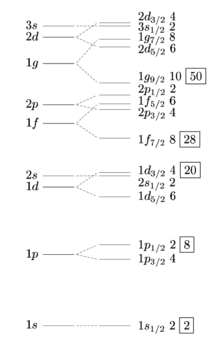
\includegraphics[width=0.45\textwidth]{TeX_files/NuclearShells}
\caption[Nuclear Shell Model level diagram]{From Wikipedia: "Low-lying energy levels in a single-particle shell model with an oscillator potential (with a small negative l2 term) without spin-orbit (left) and with spin-orbit (right) interaction. The number to the right of a level indicates its degeneracy, (2j+1). The boxed integers indicate the magic numbers."}
\label{fig:NuclearShells}
\end{wrapfigure}

Now imagine you stretch out the nucleus somehow. That'll certainly change the spacing and position of the energy levels, because some electron orbitals have a sort of intrinsic shape characteristic that might be better- or worse-suited for the new elongation.

Finally, imagine that you do the stretching \textit{continuously}. That is what is done in a Nilsson diagram. For example, in figure \ref{fig:NilssonDiagram}, the system is elongated from a spherical ground state, and the changing energy levels are the curves, which frequently end up crossing one another. An important thing to notice is that, for different deformations you might have different shell gaps, and as well you might find that different orbitals are more favorable at different deformations.

\begin{figure}
\centering
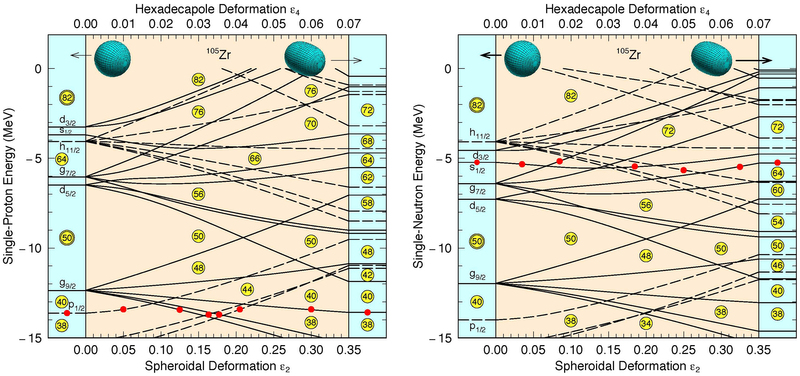
\includegraphics[width=0.7\linewidth]{TeX_files/NilssonDiagram}
\caption[Nilsson Diagram for Zr-105]{Nilsson Diagram for Zr-105, plotted against elongation parameter $\epsilon_2$}
\label{fig:NilssonDiagram}
\end{figure}

Anyway, that's all helpful \textit{once you know} the deformation. And there's a lot of useful and interesting things you can say and predict using a Nilsson diagram - heck, if you know the shape you can [qualitatively] even \textit{draw} a Nilsson diagram, just by thinking about the physical system and how the orbitals are probably behaving.  BUT if you want to understand why a nucleus deforms in the first place, that's a whole other story.

\section{What causes nuclear ground state deformations?}

As with most peculiarities of nuclear structure, the source of nuclear deformation is primarily an artifact of shell structure. In particular, when there is a large shell gap, the nucleus will get sort of "locked" into a particular stable configuration, and if that happens to be a deformed configuration because of the orbital characteristics of the outermost nucleons (because that's the only thing that could matter, right?), then so be it.

A question that I have is how is there ground state deformation in even-even nuclei? Because even-even nuclei all have, without exception, spin-parity $0^+$, and yet $^{152}Dy$ (for example) is highly-deformed. Am I misunderstanding the implications of such a spin-parity assignment? Or am I misunderstanding what is meant by "ground state deformed"?

I don't think this is a real answer, but one way to identify even-even deformed nuclei is to look for nuclei with a large $\frac{E(4^+)}{E(2^+)}$ ratio (or a related method is to look for those with a relatively-small $E(2^+)$).

\section{Phenomenology of Nilsson Diagrams}

[Basically here is where you were thinking about Casten's slides. He goes through and talks about whether a level's energy will go up or down, and how it will curve, just by thinking about the orbital motion of single particles around different axes of the deformed system.]

\section{What causes nuclear ground state deformations? Part 2}
\subsection{What causes fission?}

I think there's a couple of effects at play that lead to fission. First of all, what gets the nucleus moving in the first place, and second, what \textit{keeps} it moving?

To answer the first question, imagine you were to buy a bunch of nucleons at the store and then put them in a box together. Just dump them in with some arbitrary configuration. They'll start to attract and repel one another and there will be kind of a chaotic mess of particle motions to keep track of. TDHF will kind of give you a sense of what's going on in sort of an average sense.

Eventually, the system might settle into a set of sort of normal modes. There will probably be several overlapping normal modes happening at once, so the motion will still look pretty chaotic, but in some average sense you might get something that starts to move with some pseudo-regularity. And with time (I suppose regardless of whether the system motion os regular or not), the system might (for example) elongate, and in fact it might elongate enough for there to be a level crossing in the Nilsson diagram.

When this happens, the system has some deciding to do. It might continue on its current trajectory, or it might jump onto another trajectory (that is, there might be a nucleonic transition from one energy level to another). I suppose it is pretty difficult in practice for a nucleon to make these transitions, because you have all kind of things like conservation of angular momentum and Pauli's principle and such to consider. BUT if you transition a pair of nucleons instead of just one, you can skirt around a lot of these issues, and so I think that's what frequently tends to happen. That is why pairing correlations are sometimes called the "lubricant" of nuclear fission \cite{Bulgac2016}.

\backmatter
% bibliography, glossary and index would go here.
\bibliography{main}
\bibliographystyle{abbrv}

\end{document}